%% bare_conf_compsoc.tex
%% V1.4b
%% 2015/08/26
%% by Michael Shell
%% See:
%% http://www.michaelshell.org/
%% for current contact information.
%%
%% This is a skeleton file demonstrating the use of IEEEtran.cls
%% (requires IEEEtran.cls version 1.8b or later) with an IEEE Computer
%% Society conference paper.
%%
%% Support sites:
%% http://www.michaelshell.org/tex/ieeetran/
%% http://www.ctan.org/pkg/ieeetran
%% and
%% http://www.ieee.org/

%%*************************************************************************
%% Legal Notice:
%% This code is offered as-is without any warranty either expressed or
%% implied; without even the implied warranty of MERCHANTABILITY or
%% FITNESS FOR A PARTICULAR PURPOSE! 
%% User assumes all risk.
%% In no event shall the IEEE or any contributor to this code be liable for
%% any damages or losses, including, but not limited to, incidental,
%% consequential, or any other damages, resulting from the use or misuse
%% of any information contained here.
%%
%% All comments are the opinions of their respective authors and are not
%% necessarily endorsed by the IEEE.
%%
%% This work is distributed under the LaTeX Project Public License (LPPL)
%% ( http://www.latex-project.org/ ) version 1.3, and may be freely used,
%% distributed and modified. A copy of the LPPL, version 1.3, is included
%% in the base LaTeX documentation of all distributions of LaTeX released
%% 2003/12/01 or later.
%% Retain all contribution notices and credits.
%% ** Modified files should be clearly indicated as such, including  **
%% ** renaming them and changing author support contact information. **
%%*************************************************************************


% *** Authors should verify (and, if needed, correct) their LaTeX system  ***
% *** with the testflow diagnostic prior to trusting their LaTeX platform ***
% *** with production work. The IEEE's font choices and paper sizes can   ***
% *** trigger bugs that do not appear when using other class files.       ***                          ***
% The testflow support page is at:
% http://www.michaelshell.org/tex/testflow/



\documentclass[conference,compsoc]{IEEEtran}
% Some/most Computer Society conferences require the compsoc mode option,
% but others may want the standard conference format.
%
% If IEEEtran.cls has not been installed into the LaTeX system files,
% manually specify the path to it like:
% \documentclass[conference,compsoc]{../sty/IEEEtran}





% Some very useful LaTeX packages include:
% (uncomment the ones you want to load)


% *** MISC UTILITY PACKAGES ***
%
%\usepackage{ifpdf}
% Heiko Oberdiek's ifpdf.sty is very useful if you need conditional
% compilation based on whether the output is pdf or dvi.
% usage:
% \ifpdf
%   % pdf code
% \else
%   % dvi code
% \fi
% The latest version of ifpdf.sty can be obtained from:
% http://www.ctan.org/pkg/ifpdf
% Also, note that IEEEtran.cls V1.7 and later provides a builtin
% \ifCLASSINFOpdf conditional that works the same way.
% When switching from latex to pdflatex and vice-versa, the compiler may
% have to be run twice to clear warning/error messages.






% *** CITATION PACKAGES ***
%
\ifCLASSOPTIONcompsoc
  % IEEE Computer Society needs nocompress option
  % requires cite.sty v4.0 or later (November 2003)
  \usepackage[nocompress]{cite}
\else
  % normal IEEE
  \usepackage{cite}
\fi
% cite.sty was written by Donald Arseneau
% V1.6 and later of IEEEtran pre-defines the format of the cite.sty package
% \cite{} output to follow that of the IEEE. Loading the cite package will
% result in citation numbers being automatically sorted and properly
% "compressed/ranged". e.g., [1], [9], [2], [7], [5], [6] without using
% cite.sty will become [1], [2], [5]--[7], [9] using cite.sty. cite.sty's
% \cite will automatically add leading space, if needed. Use cite.sty's
% noadjust option (cite.sty V3.8 and later) if you want to turn this off
% such as if a citation ever needs to be enclosed in parenthesis.
% cite.sty is already installed on most LaTeX systems. Be sure and use
% version 5.0 (2009-03-20) and later if using hyperref.sty.
% The latest version can be obtained at:
% http://www.ctan.org/pkg/cite
% The documentation is contained in the cite.sty file itself.
%
% Note that some packages require special options to format as the Computer
% Society requires. In particular, Computer Society  papers do not use
% compressed citation ranges as is done in typical IEEE papers
% (e.g., [1]-[4]). Instead, they list every citation separately in order
% (e.g., [1], [2], [3], [4]). To get the latter we need to load the cite
% package with the nocompress option which is supported by cite.sty v4.0
% and later.





% *** GRAPHICS RELATED PACKAGES ***
%
\ifCLASSINFOpdf
  \usepackage[pdftex]{graphicx}
  % declare the path(s) where your graphic files are
  % \graphicspath{{../pdf/}{../jpeg/}}
  % and their extensions so you won't have to specify these with
  % every instance of \includegraphics
  % \DeclareGraphicsExtensions{.pdf,.jpeg,.png}
\else
  % or other class option (dvipsone, dvipdf, if not using dvips). graphicx
  % will default to the driver specified in the system graphics.cfg if no
  % driver is specified.
  % \usepackage[dvips]{graphicx}
  % declare the path(s) where your graphic files are
  % \graphicspath{{../eps/}}
  % and their extensions so you won't have to specify these with
  % every instance of \includegraphics
  % \DeclareGraphicsExtensions{.eps}
\fi
% graphicx was written by David Carlisle and Sebastian Rahtz. It is
% required if you want graphics, photos, etc. graphicx.sty is already
% installed on most LaTeX systems. The latest version and documentation
% can be obtained at: 
% http://www.ctan.org/pkg/graphicx
% Another good source of documentation is "Using Imported Graphics in
% LaTeX2e" by Keith Reckdahl which can be found at:
% http://www.ctan.org/pkg/epslatex
%
% latex, and pdflatex in dvi mode, support graphics in encapsulated
% postscript (.eps) format. pdflatex in pdf mode supports graphics
% in .pdf, .jpeg, .png and .mps (metapost) formats. Users should ensure
% that all non-photo figures use a vector format (.eps, .pdf, .mps) and
% not a bitmapped formats (.jpeg, .png). The IEEE frowns on bitmapped formats
% which can result in "jaggedy"/blurry rendering of lines and letters as
% well as large increases in file sizes.
%
% You can find documentation about the pdfTeX application at:
% http://www.tug.org/applications/pdftex





% *** MATH PACKAGES ***
%
%\usepackage{amsmath}
% A popular package from the American Mathematical Society that provides
% many useful and powerful commands for dealing with mathematics.
%
% Note that the amsmath package sets \interdisplaylinepenalty to 10000
% thus preventing page breaks from occurring within multiline equations. Use:
%\interdisplaylinepenalty=2500
% after loading amsmath to restore such page breaks as IEEEtran.cls normally
% does. amsmath.sty is already installed on most LaTeX systems. The latest
% version and documentation can be obtained at:
% http://www.ctan.org/pkg/amsmath





% *** SPECIALIZED LIST PACKAGES ***
%
%\usepackage{algorithmic}
% algorithmic.sty was written by Peter Williams and Rogerio Brito.
% This package provides an algorithmic environment fo describing algorithms.
% You can use the algorithmic environment in-text or within a figure
% environment to provide for a floating algorithm. Do NOT use the algorithm
% floating environment provided by algorithm.sty (by the same authors) or
% algorithm2e.sty (by Christophe Fiorio) as the IEEE does not use dedicated
% algorithm float types and packages that provide these will not provide
% correct IEEE style captions. The latest version and documentation of
% algorithmic.sty can be obtained at:
% http://www.ctan.org/pkg/algorithms
% Also of interest may be the (relatively newer and more customizable)
% algorithmicx.sty package by Szasz Janos:
% http://www.ctan.org/pkg/algorithmicx




% *** ALIGNMENT PACKAGES ***
%
%\usepackage{array}
% Frank Mittelbach's and David Carlisle's array.sty patches and improves
% the standard LaTeX2e array and tabular environments to provide better
% appearance and additional user controls. As the default LaTeX2e table
% generation code is lacking to the point of almost being broken with
% respect to the quality of the end results, all users are strongly
% advised to use an enhanced (at the very least that provided by array.sty)
% set of table tools. array.sty is already installed on most systems. The
% latest version and documentation can be obtained at:
% http://www.ctan.org/pkg/array


% IEEEtran contains the IEEEeqnarray family of commands that can be used to
% generate multiline equations as well as matrices, tables, etc., of high
% quality.




% *** SUBFIGURE PACKAGES ***
%\ifCLASSOPTIONcompsoc
%  \usepackage[caption=false,font=footnotesize,labelfont=sf,textfont=sf]{subfig}
%\else
%  \usepackage[caption=false,font=footnotesize]{subfig}
%\fi
% subfig.sty, written by Steven Douglas Cochran, is the modern replacement
% for subfigure.sty, the latter of which is no longer maintained and is
% incompatible with some LaTeX packages including fixltx2e. However,
% subfig.sty requires and automatically loads Axel Sommerfeldt's caption.sty
% which will override IEEEtran.cls' handling of captions and this will result
% in non-IEEE style figure/table captions. To prevent this problem, be sure
% and invoke subfig.sty's "caption=false" package option (available since
% subfig.sty version 1.3, 2005/06/28) as this is will preserve IEEEtran.cls
% handling of captions.
% Note that the Computer Society format requires a sans serif font rather
% than the serif font used in traditional IEEE formatting and thus the need
% to invoke different subfig.sty package options depending on whether
% compsoc mode has been enabled.
%
% The latest version and documentation of subfig.sty can be obtained at:
% http://www.ctan.org/pkg/subfig




% *** FLOAT PACKAGES ***
%
%\usepackage{fixltx2e}
% fixltx2e, the successor to the earlier fix2col.sty, was written by
% Frank Mittelbach and David Carlisle. This package corrects a few problems
% in the LaTeX2e kernel, the most notable of which is that in current
% LaTeX2e releases, the ordering of single and double column floats is not
% guaranteed to be preserved. Thus, an unpatched LaTeX2e can allow a
% single column figure to be placed prior to an earlier double column
% figure.
% Be aware that LaTeX2e kernels dated 2015 and later have fixltx2e.sty's
% corrections already built into the system in which case a warning will
% be issued if an attempt is made to load fixltx2e.sty as it is no longer
% needed.
% The latest version and documentation can be found at:
% http://www.ctan.org/pkg/fixltx2e


%\usepackage{stfloats}
% stfloats.sty was written by Sigitas Tolusis. This package gives LaTeX2e
% the ability to do double column floats at the bottom of the page as well
% as the top. (e.g., "\begin{figure*}[!b]" is not normally possible in
% LaTeX2e). It also provides a command:
%\fnbelowfloat
% to enable the placement of footnotes below bottom floats (the standard
% LaTeX2e kernel puts them above bottom floats). This is an invasive package
% which rewrites many portions of the LaTeX2e float routines. It may not work
% with other packages that modify the LaTeX2e float routines. The latest
% version and documentation can be obtained at:
% http://www.ctan.org/pkg/stfloats
% Do not use the stfloats baselinefloat ability as the IEEE does not allow
% \baselineskip to stretch. Authors submitting work to the IEEE should note
% that the IEEE rarely uses double column equations and that authors should try
% to avoid such use. Do not be tempted to use the cuted.sty or midfloat.sty
% packages (also by Sigitas Tolusis) as the IEEE does not format its papers in
% such ways.
% Do not attempt to use stfloats with fixltx2e as they are incompatible.
% Instead, use Morten Hogholm'a dblfloatfix which combines the features
% of both fixltx2e and stfloats:
%
% \usepackage{dblfloatfix}
% The latest version can be found at:
% http://www.ctan.org/pkg/dblfloatfix




% *** PDF, URL AND HYPERLINK PACKAGES ***
%
\usepackage{url}
% url.sty was written by Donald Arseneau. It provides better support for
% handling and breaking URLs. url.sty is already installed on most LaTeX
% systems. The latest version and documentation can be obtained at:
% http://www.ctan.org/pkg/url
% Basically, \url{my_url_here}.




% *** Do not adjust lengths that control margins, column widths, etc. ***
% *** Do not use packages that alter fonts (such as pslatex).         ***
% There should be no need to do such things with IEEEtran.cls V1.6 and later.
% (Unless specifically asked to do so by the journal or conference you plan
% to submit to, of course. )


% correct bad hyphenation here
\hyphenation{op-tical net-works semi-conduc-tor}
\usepackage[portuguese]{babel}
\usepackage{multirow}

\begin{document}
%
% paper title
% Titles are generally capitalized except for words such as a, an, and, as,
% at, but, by, for, in, nor, of, on, or, the, to and up, which are usually
% not capitalized unless they are the first or last word of the title.
% Linebreaks \\ can be used within to get better formatting as desired.
% Do not put math or special symbols in the title.
\title{Recomendação de Algoritmos em Fluxos de Dados}


% author names and affiliations
% use a multiple column layout for up to three different
% affiliations
\author{\IEEEauthorblockN{Jáder Martins Camboim de Sá}
\IEEEauthorblockA{Departamento de Ciência da Computação\\
Universidade de Brasília\\
Brasilia, Brasil 70910-900\\
Email: jader.martins@ipea.gov.br}
\and
\IEEEauthorblockN{Luís Paulo Faina Garcia}
\IEEEauthorblockA{Departamento de Ciência da Computação\\
Universidade de Brasília\\
Brasilia, Brasil 70910-900\\
Email: luis.garcia@unb.br}}

\maketitle


\begin{abstract}
Em ambientes dinâmicos, como fluxos de dados, modelos estáticos costumam perecer apresentando performances cada vez piores ao longo do tempo. O retreinamento de modelos é uma prática comum na solução desse problema, porém em casos de mudanças abruptas a escolha de um novo algorimo pode ser mais adequado. Nesse trabalho, apresentamos um aprimoramento do MetaStream para seleção de algoritmos em fluxos de dados. Nossa abordagem usa de meta-atributos do estado-da-arte combinado a um aprendizado incremental para selecionar efetivamente o melhor algoritmo a ser usado em dados que mudam com o tempo.
\end{abstract}

\IEEEpeerreviewmaketitle

\section{Introdução}
\label{intro}
A produção de dados em alta frequência é cada mais comum por tecnologias e dispositivos que interagem com os humanos. Diversas companhias, como Google, Apple e Samsung tem incentivado e explorado o potencial que essa quantidade massiva de informação pode prover pela mineração de dados \cite{tarnoff2018big}.
Exemplos de aplicações são assistentes pessoais, que recomendam o melhor momento para ir para casa e evitar transito, músicas para se ouvir de acordo com seus preferências mais recentes, ou até mesmo ligar para seu médico caso seu smartwatch detecte alguma variação indevida no ritmo cardíaco.

Dentre as metodologias de mineração de dados, o Aprendizado de Máquina (AM), é uma das áreas de pesquisa que se sobressai em relação as seus resultados, beneficiado pela ``eficácia irracional dos dados'' \cite{halevy2009unreasonable}. O AM visa extrair padrões dos dados presentes para que possa inferir características em eventos futuros \cite{mitchell1997machine}, porém, essa abordagem assume premissas indutivas que nem sempre se mantém, tornando a abordagem tradicional de AM inviável em que a distribuição dos dados muda com o tempo \cite{gama2007learning}.

A maioria das abordagens de fluxos de dados, se baseia em um modelo ou um comitê de modelos com o mesmo classificador a nível base. Essa abordagem assume que um único espaço de hipóteses é o melhor para qualquer conceito que venha a surgir nos dados. Entretanto, nós obtemos mais poder preditivo aprendendo conceitos distintos por diferentes paradigmas de aprendizado \cite{rossi2014metastream}. O problema central é então é como eficientemente escolher o algoritmo de aprendizado mais apropriado dado uma amostra de dados.

O Meta-Aprendizado, é uma técnica que visa aprender e inferir algum aspecto do processo de AM através de meta-exemplos, inicialmente são extraídas características descritiva para o problema em questão e em seguida são definidos os atributos alvo a serem aprendidos, que para o problema aqui em questão é qual espaço de hipótese será mais adequado para uma dada distribuição.

Nesse trabalho nós aprimoramos o MetaStream \cite{rossi2014metastream}, pelo aumento do conjunto de meta-atributos descritivos para um conjunto estado-da-arte \cite{rivolli2018towards}, e também propomos o aprendizado incremental usando o algoritmo LightGBM \cite{ke2017lightgbm} como meta-classificador. Na Seção \ref{method}, detalhamos o funcionamento do MetaStream e os meta-atributos selecionados para o experimento, na Seção \ref{result} apresentamos e analisamos os resultados com fim de selecionar efetivamente algoritmos em momentos futuros, e por fim, na Seção \ref{conclusion}, concluímos esse trabalho.


\section{Metodologia}
\label{method}
O problema de seleção de algoritmos aqui proposto, consiste em selecionar o algoritmo com espaço de hipóteses mais adequado para o fluxo de dados em um momento futuro a partir de instâncias observadas no fluxo atual, esse modelo é denominado MetaStream, proposto em \cite{rossi2014metastream}. Na Subseção \ref{metastream} descrevemos o \textit{framework} utilizado, na Subseção \ref{configs} descrevemos as medidas de informação extraídas dos dados, algoritmos utilizados e parâmetros do \textit{framework} e na Subseção \ref{datasets} descrevemos os conjuntos de dados utilizados para avaliar o experimento.

\subsection{MetaStream}
\label{metastream}
Inicialmente observamos o fluxo de dados até que uma quantidade significativa de exemplos seja adiquirida. Com esse lote de dados, o MetaStream induz algoritmos base por meio de uma validação cruzada \textit{k-fold} para seleção de hiperparametros. Em seguida, o algoritmo realiza uma janelamento sobre os dados, como mostrado na Figura \ref{fig:ms_diag0_off}. Para a janela $\omega_{b1}$ são extraídas os meta-atributos $x^m$ do meta-exemplo 1 e também é usada para treinar os algoritmos nível base, para a janela $\eta_{b1}$ os algoritmos anteriormente treinados são avaliados e o de melhor performance é definido como a etiqueta do meta-exemplo 1, $y^m$. Realizando esse processo deslizando $\eta_b$ exemplos.

\begin{figure}[ht]
    \centering
    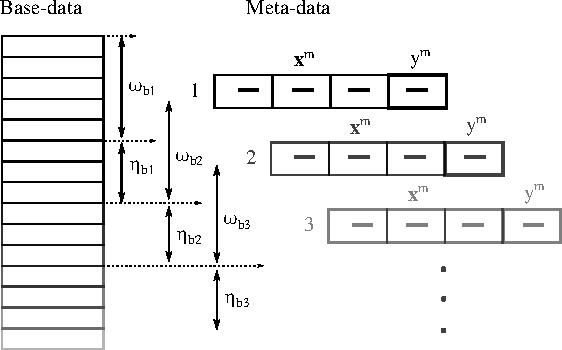
\includegraphics[width=\linewidth]{imgs/ms_diag0_off.pdf}
    \caption{Extração de meta-atributos da janela $\omega_{bn}$ e obtenção da etiqueta da janela $\eta_{bn}$.}
    \label{fig:ms_diag0_off}
\end{figure}

Após realizado $n$ etapas, na Figura \ref{fig:ms_diagram1} exemplificado como $n=40$, é construída uma meta-base, essa meta-base é usada para induzir modelos usando o meta-classificador que irá recomendar algoritmos a serem usadas nas próximas janelas. Ao chegar uma nova janela $\omega_b$, com os exemplos etiquetados, é extraída o vetor $x^m$ do meta-exemplo 41, esse vetor $x^m$ é então usado para prever a etiqueta $y^m$, isto é, recomendar o algoritmo que foi treinado na janela $\omega_b$ que melhor preverá os exemplos da janela $\eta_b$.

\begin{figure}[ht]
    \centering
    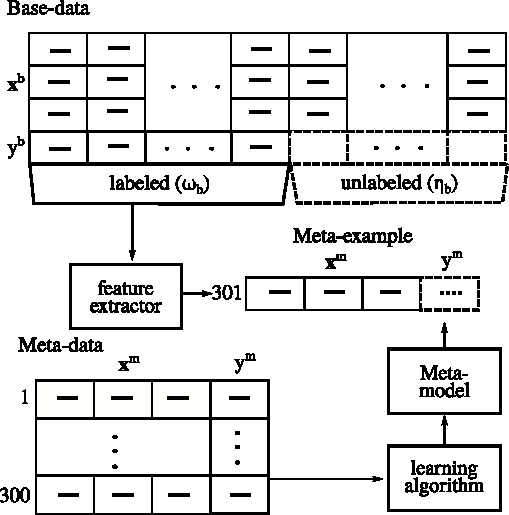
\includegraphics[width=\linewidth]{imgs/metastream_diag1.pdf}
    \caption{Meta-feature extraction from $\omega_b$ and $\eta_b$ windows at meta-level.}
    \label{fig:ms_diagram1}
\end{figure}

Após algum intervalo variável, as etiquetas da janela $\eta_b$ são obtidos e definidos para está mesma janela como treino, com isso também é possível mensurar as performances a nível base dos algoritmos e definir a real etiqueta $y^m$ do exemplo 41, este que é posteriormente adicionado a meta-base.

\subsection{Configurações e Parâmetros}
\label{configs}
Para a escolha de algoritmos do nível base levamos alguns fatores em consideração, a capacidade preditiva, custo computacional e diversidade de espaço de hipóteses, com isso dois algoritmos foram selecionados, o Random Forest (RF) \cite{breiman2001random} e um aproximação eficiente do RBF-SVM através do método de Nystr\"oem \cite{williams2001using}. Já para o meta-classificador, isto é, o algoritmo que irá realizar a recomendação, escolhemos o LightGBM, analogamente as quesitos anteriores e também sua capacidade de aprendizado incremental.

Para os meta-atributos, três grupos foram selecionados, chamados \textit{statistical}, \textit{model-based} e \textit{landmarking}. Em geral esses grupos possuem alta capacidade discriminativa e um baixo custo computacional \cite{rivolli2018towards}. Esses meta-atributos foram extraídos usando a biblioteca Python Meta-Feature Extractor (pymfe) \cite{pymfe2020}  disponível publicamente no GitHub\footnote{\url{https://github.com/ealcobaca/pymfe}}.

Nós fixamos os tamanhos de janelas para todos os experimentos, em nível base e nível meta definimos $\omega_{m;b} = 300$ e $\eta_{m;b} = 10$, e o passo da janela de treinamento é o mesmo que $\eta$. Após os parâmetros terem sido selecionados como descrito na Seção \ref{metastream}, eles são mantidos durante todo o experimento. Por fim, as performances são mensuradas pelas métricas acurácia (Acc), Kappa score e Média Geométrica (GMean), tanto na fase online quanto offline.

\subsection{Conjuntos de Dados}
\label{datasets}

Para os experimentos, nós selecionamos três conjuntos de dados de classificação populares na literatura de fluxo de dados que apresentam mudança de conceito. Esses conjunto de dados são gerados sinteticamente utilizando da biblioteca \textit{skmultiflow} \cite{skmultiflow}, para os três conjuntos foram gerados 40000 exemplos.

\begin{itemize}
\item{\textit{HyperPlane:}} Esse conjunto é construído inicialmente criando um hiperplano $d$-dimensional, dado pelo vetor $w$, e pontos aleatórios são definidos nesse espaço, pontos no sentido do vetor são positivos e abaixo dele negativos, criando um problema de classificação binária, esse vetor é então rotacionado por uma aceleração variante, causando então a mudança de conceito.

\item{\textit{Agrawal:}} Esse fluxo de dados contém 9 atributos preditivos, sendo 6 numéricos e 3 categóricos. Como tarefa uma das funções descrita em \cite{agrawal1993database} define se um cliente deve ou não ter seu crédito aprovado. A mudança de conceito é causada pela mudança da função que determina a fraude de crédito.

\item{\textit{RandomRBF:}} O Função de Base Radial Aleatória (Random Radial Basis Function) gera um conjunto de dados criando um centroide para cada classe, cada centro gerado aleatoriamente é movido com certa aceleração. Para gerar novas instâncias, um centro é escolhido aleatoriamente a partir de seus pesos e os atributos são aleatoriamente gerados deslocados do centroide, este que determina a classe da instância.
\end{itemize}

A analise dos experimentos é dividida em fases offline e online. A fase offline analisa o \textit{framework} no nível meta, isto é, o quão bem ele pode prever o melhor algoritmo. A fase online analise em nível base, onde são comparados os ganhos obtidos por recomendar um algoritmo, contra o método sem recomendação, aquele em que se usa o algoritmo que teve melhor performance durante a fase de validação, esse método é chamado daqui em diante de \textit{Default}.

\section{Resultados}
\label{result}

A Tabela \ref{tab:algo_dist} lista a distribuição dos algoritmos (RF e SVM\footnote{Uma aproximação do SVM como descrito na seção anterior.}) que apresentaram as melhores performances para cada janela na meta-base. Na perspectiva de MtA, essa tabela apresenta a distribuição de classes para os meta-exemplos.

\begin{table}[ht]
\caption{Distribuição de algoritmos nos meta-dados por problema de fluxo de dados.}
\label{tab:algo_dist}
\centering
\begin{tabular}{r|c|c}
    Conjunto de Dados & SVM   & RF    \\ \hline
    HyperPlane        & 0.792 & 0.207 \\
    Agrawal           & 0.785 & 0.215 \\
    RandomRBF         & 0.535 & 0.465 \\
\end{tabular}
\end{table}

Para os três conjuntos de dados, o SVM teve uma melhor performance, sendo que para o HyperPlane e o Agrawal a distribuição tende significativamente para o SVM, dado essa condição, configuramos o meta-classificador balancear entre as classes quando for induzir modelos. O algoritmo Default é aquele que domina a distribuição nessa primeira fase, logo para todos eles temos o SVM como Default.

Em seguida avaliamos o meta-classificador em uma validação de series temporais, respeitando a ordem em que as instâncias foram observadas, na mesma configuração de janelamento definida na Subseção \ref{configs}. Na Tabela \ref{tab:offmetrics} são reportados as métricas obtidas nesta avaliação.

\begin{table}[ht]
\caption{Performance preditiva do meta-classificador na fase offline.}
\label{tab:offmetrics}
\centering
\begin{tabular}{r|c|c|c}
    Fluxo   & Kappa           & M. Geométrica   & Acurácia        \\ \hline
HyperPlane  & 0.118$\pm$0.326 & 0.120$\pm$0.325 & 0.841$\pm$0.080 \\
Agrawal     & 0.007$\pm$0.138 & 0.046$\pm$0.164 & 0.780$\pm$0.078 \\
RandomRBF   & 0.120$\pm$0.239 & 0.416$\pm$0.262 & 0.571$\pm$0.115 \\
\end{tabular}
\end{table}

Embora não se tenha valores de Kappa altos, dado pelo fato da grande maioria dos meta-exemplos representarem na verdade um empate para aquela janela, eles são ligeiramente positivos para todos os conjuntos de dados, isso representa que a recomendação, em média, não é pior que o default, esse que teria um Kappa de zero.

Na Tabela \ref{tab:onmetrics}, são reportados os resultados dos experimentos online, onde as estratégias incrementais e não-incrementais são avaliadas.

\begin{table}[ht]
\caption{Performance preditiva do meta-classificador na fase online.}
\label{tab:onmetrics}
\centering
\begin{tabular}{r|l|c|c|c}
Conjunto     &  Estratégia    & Kappa & GMean & Acc \\ \hline
\multirow{2}{*}{HyperPlane}   &  Non-Incremental       & 0.014 & 0.265  & 0.747    \\
            &  Incremental & 0.020 & 0.283  & 0.745    \\ \hline
\multirow{2}{*}{Agrawal}   &  Non-Incremental       & 0.010 & 0.198  & 0.794    \\
            &  Incremental & -0.041 & 0.327  & 0.700    \\ \hline
\multirow{2}{*}{RandomRBF}   &  Non-Incremental       & -0.031 & 0.484  & 0.484    \\
            &  Incremental & 0.004 & 0.486  & 0.501
\end{tabular}
\end{table}

Embora os resultados não sejam positivos para o experimento online em algumas combinações conjunto-estratégia, apenas essas métricas não contam a historia completa, pois como descrito anteriormente há pontos de empate e pontos que tem uma maior ganho pela escolha que não são capturados por essas métricas, mas que sua qualidade será apresentada pelas Figuras de 3 a 8.

Nas Figuras de \ref{fig:cumsum_hyper} a \ref{fig:cumsum_rbf} é apresentado o ganho de performance acumulado para as diferentes combinações de estratégia-conjunto de dados. Os pontos pretos representa a diferença de score, no momento $t$, entre o algoritmo recomendado e o algoritmo Default.
% Se o ponto preto estiver acima do eixo $y=0$ significa que houve um ganho pela recomendação de algoritmo, ou seja o RF teve uma performance melhor que o SVM para aquela janela $t$, se o ponto estiver abaixo da linha houve um perda por recomendação, se o ponto estiver exatamente na linha, não houveram ganhos ou perdas.
Também é apresentada uma região preenchida representado o somatório acumulado de ganhos e perdas ao longo do tempo, em laranja para a estratégia não-incremental e em azul para a estratégia incremental.

\begin{figure}[ht]
    \centering
    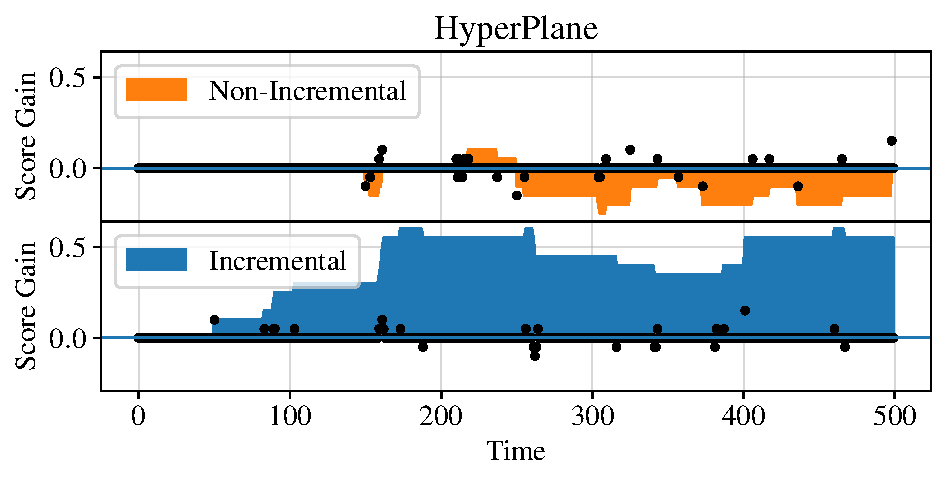
\includegraphics[width=\linewidth]{imgs/hyper_cumsum.pdf}
    \caption{Ganho cumulativo de performance para o HyperPlane.}
    \label{fig:cumsum_hyper}
\end{figure}

\begin{figure}[ht]
    \centering
    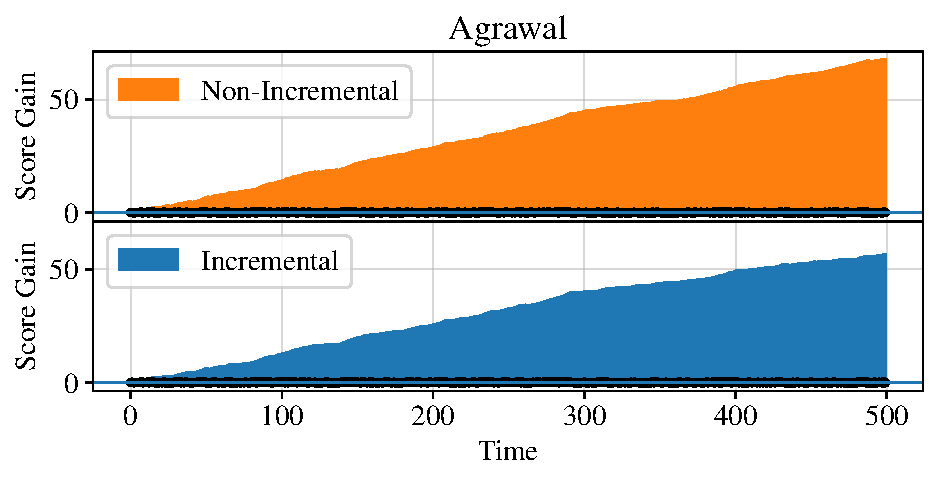
\includegraphics[width=\linewidth]{imgs/agrawal_cumsum.pdf}
    \caption{Ganho cumulativo de performance para o Agrawal.}
    \label{fig:cumsum_agrawal}
\end{figure}

\begin{figure}[ht]
    \centering
    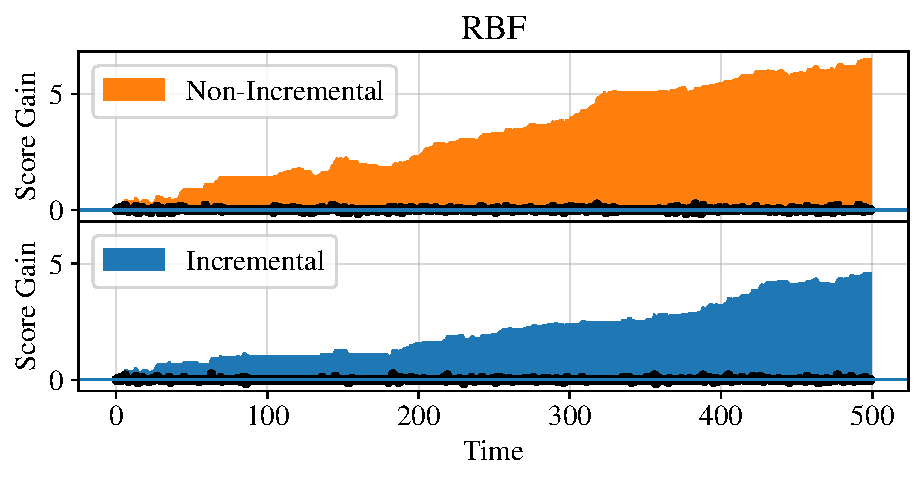
\includegraphics[width=\linewidth]{imgs/rbf_cumsum.pdf}
    \caption{Ganho cumulativo de performance para o RBF.}
    \label{fig:cumsum_rbf}
\end{figure}

Para os 3 conjuntos de dados o \textit{framework} conseguiu desempenhar ganhos positivos para a estratégia incremental, já para a não-incremental, apresentou uma performance ruim para o conjunto de dados HyperPlane, sendo as possíveis causas o sobre-ajuste ou esquecimento de conceitos.


\begin{figure}[ht]
    \centering
    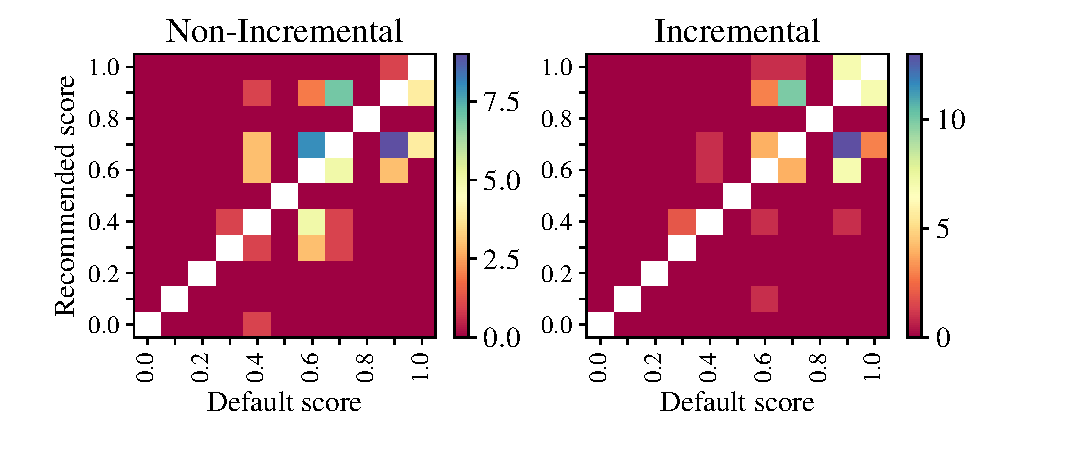
\includegraphics[width=\linewidth]{imgs/hyper_score.pdf}
    \caption{Comparação entre o método recomendado e o Default (HyperPlane).}
    \label{fig:cross_score_hyper}
\end{figure}

\begin{figure}[ht]
    \centering
    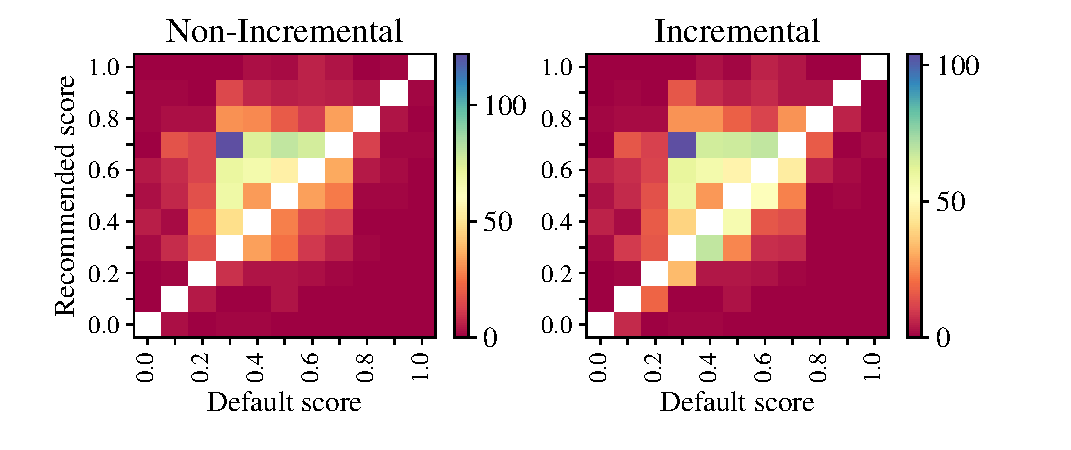
\includegraphics[width=\linewidth]{imgs/agrawal_score.pdf}
    \caption{Comparação entre o método recomendado e o Default (Agrawal).}
    \label{fig:cross_score_agrawal}
\end{figure}


\begin{figure}[ht!]
    \centering
    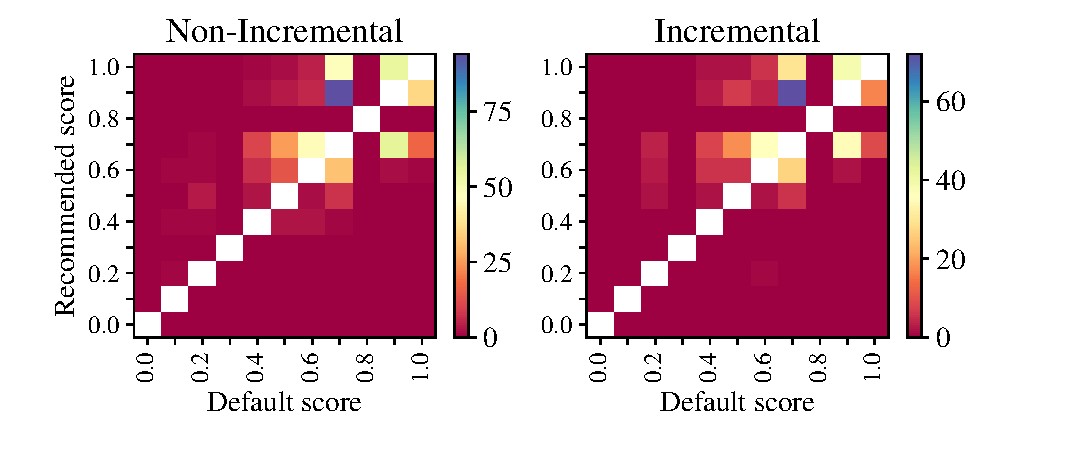
\includegraphics[width=\linewidth]{imgs/rbf_score.pdf}
    \caption{Comparação entre o método recomendado e o Default (RBF).}
    \label{fig:cross_score_rbf}
\end{figure}


\section{Conclusão}
\label{conclusion}

Nesse trabalho, apresentamos um método baseado em MtA sob um aprimoramento do \textit{framework} original, o MetaStream. As melhorias foram através de meta-atributos mais modernos e mais informativos e pela inclusão de uma abordagem incremental baseada no algoritmo LightGBM como meta-classificador.

Embora ambas as estratégias tenham tido uma performance similar, para o conjunto \textit{HyperPlane} a possibilidade de lembrar conceitos passados fez com que a performance fosse positiva em pontos mais avançados no tempo. Além disso, o algoritmo incremental apresenta um consumo menor de memória e menos tempo para processamento de indução de modelo, sendo então uma abordagem mais adequada quando esses fatores são criticos a aplicação.

A estratégia incremental para todos os conjuntos de dados, conseguiu sistematicamente recomendar o melhor algoritmo para uma dada janela no fluxo de dados, levando a um ganho crescente de performance ao longo do tempo.

% Como trabalho futuros, gostaríamos de implementar o processo de extração de meta-atributos incremental, possibilitando adicionar grupos de meta-atributos mais robustos quanto a capacidade discriminativa. Também, como o artigo original propõem  \cite{rossi2014metastream}, atributos baseados em series temporais podem ajudar significativamente na previsão, sendo uma boa abordagem para os próximos trabalhos.


% \ifCLASSOPTIONcompsoc
%   % The Computer Society usually uses the plural form
%   \section*{Agradecimentos}
% \else
%   % regular IEEE prefers the singular form
%   \section*{Agradecimento}
% \fi



\bibliographystyle{IEEEtran}
\bibliography{ref.bib}

\end{document}


